      
               
                \begin{ledgroupsized}[r]{120mm}
                \footnotesize 
                \pstart                
                \noindent\textbf{\"{U}berlieferung:}   
                \pend
                \end{ledgroupsized}
            
              
                            \begin{ledgroupsized}[r]{114mm}
                            \footnotesize 
                            \pstart \parindent -6mm
                            \makebox[6mm][l]{\textit{L}}Konzept: LH XXXV 15, 6 Bl. 56. 1 Bl. rechteckig beschnitten, 10 x 17 cm. 1 S. zweispaltig. Die Zeichnung \textit{[Fig. 1]} in der oberen H\"{a}lfte der linken Spalte, die anderen Zeichnungen am oberen Rand der rechten Spalte.\\KK 1, Nr. 193 K \pend
                            \end{ledgroupsized}
                %\normalsize
                \vspace*{5mm}
                \begin{ledgroup}
                \footnotesize 
                \pstart
            \noindent\footnotesize{\textbf{Datierungsgr\"{u}nde}: Der vorliegende Text weist inhaltliche Gemeinsamkeiten mit N. 3 auf. In beiden F\"{a}llen wird nach M\"{o}glichkeiten gesucht, Messungen auf See von \"{a}ußeren Einflussfaktoren unabh\"{a}ngig zu machen. Aufgrund dieser \"{U}bereinstimmungen und der Tatsache, dass es sich um Papier handelt, das Leibniz vor seiner Abreise nach Paris benutzt hat, \"{u}bernehmen wir die Datierung von N. 4.}
                \pend
                \end{ledgroup}
            
                \vspace*{8mm}
                \pstart 
                \normalsize
            [56 r\textsuperscript{o}] Sunto duo \edtext{pendula\protect\index{Sachverzeichnis}{pendulum}}{\lemma{}\Afootnote{pendula  \textbar\ rigida \textit{ gestr.}\ \textbar\ \textit{ab}, \textit{ L}}} \textit{ab}, \textit{bc} pendentia ex eodem tecto\protect\index{Sachverzeichnis}{tectum} \textit{ac}. Pone tectum\protect\index{Sachverzeichnis}{tectum} esse in loco instabili, e. g. super aquam. Efficiendum est ut duo \edtext{haec pendula}{\lemma{duo}\Afootnote{ \textit{ (1) }\ haec perpendicula sint \textit{q} \textit{ (2) }\ haec pendula \textit{ L}}} nunquam dimoveantur a situ perpendiculari ad horizontem. \edtext{Igitur}{\lemma{horizontem.}\Afootnote{ \textit{ (1) }\ Principio \textit{ (2) }\ Igitur \textit{ L}}} efficiendum est ut lineae \textit{ab}, et \textit{cd} (seu \edtext{ipsi funes}{\lemma{(seu}\Afootnote{ \textit{ (1) }\ ipsa pendula\protect\index{Sachverzeichnis}{pendulum|textit} \textit{ (2) }\ ipsi funes \textit{ L}}}) sint semper parallelae, quippe eundem angulum facientes, nempe rectum, ad idem planum, nempe horizontem, item \edtext{lineae}{\lemma{item}\Afootnote{ \textit{ (1) }\ maneant \textit{ (2) }\ lineae \textit{ L}}} \textit{ac} et \textit{bd}. Sed hoc fit etiam in non pendulis\protect\index{Sachverzeichnis}{pendulum} sed rigidis. Ergo efficiendum, ut \textit{ab} et \textit{cd} cum \textit{ac} non moveantur omnia haec fient si \textit{ab}, \textit{cd}, \textit{bd} sint acus ferreae\protect\index{Sachverzeichnis}{acus!magnetica} non firmatae, nisi per adhaerentiam magneticam, et quidem ut minus sequatur vitro interjecto. Tollet aliquas vacillationes haec methodus, (etiamsi simplici artificio pendula\protect\index{Sachverzeichnis}{pendulum} sint rigida, modis ubique connexis) irregulariores nempe quibus quodlibet, a quolibet abit, non omnes tamen nihil enim prohibet aliquamdiu immobilia, sequi tecti\protect\index{Sachverzeichnis}{tectum} inclinationem\protect\index{Sachverzeichnis}{inclinatio} quasi affixa ob celeritatem\protect\index{Sachverzeichnis}{celeritas} ictus\protect\index{Sachverzeichnis}{ictus}. \edtext{Sed si plura talia sint sub se invicem omnium minime in ultimum et forte vix sensibiliter pertinget effectus.}{\lemma{}\Afootnote{Sed [...] effectus. \textit{ erg.} \textit{ L}}}\pend \newpage \pstart  Quid? an forte Sinclari\protect\index{Namensregister}{\textso{Sinclair} (Sinclarus), George ?\textendash 1696} observatio adhiberi potest Mercurii\protect\index{Sachverzeichnis}{mercurius} ubi Tubus inclinatur, sursum resurgentis, atque impingentis in aliquid quod inclinationem\protect\index{Sachverzeichnis}{inclinatio} statim initio sistit.\pend \pstart An res procedit si instrumentum sit in ampulla tota aqua plena, quae concussione non turbatur, in cujus medio natet secundum \edtext{regulas Kircheri.\protect\index{Namensregister}{\textso{Kircher} (Kircherus), Athanasius SJ 1602\textendash 1680}}{\lemma{regulas}\Bfootnote{\textsc{A. Kircher}, \cite{00067}\textit{Magnes}, Rom 1654, S.~70\textendash 75.\protect\rule[0mm]{50mm}{0mm}}}\pend
              \begin{center}
              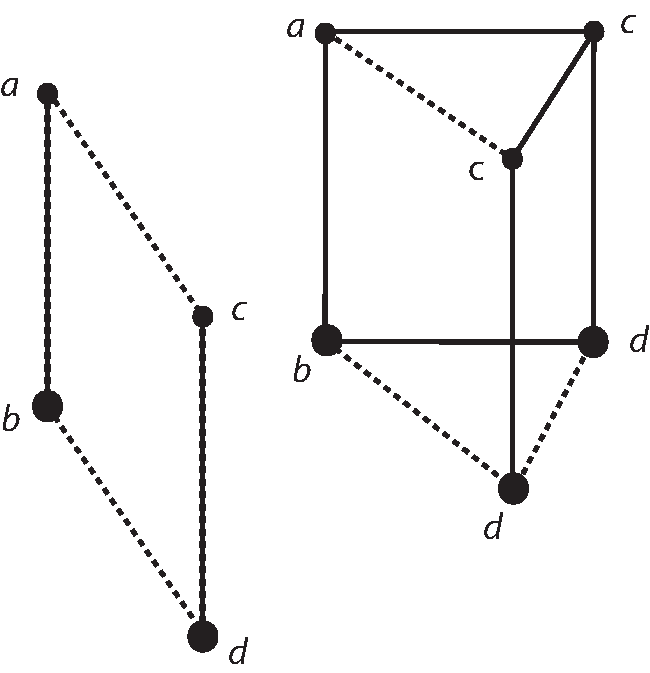
\includegraphics[width=0.4\textwidth]{images/35_15_6_56r1}\\
              \textit{[Fig. 1]}\\
              \vspace{2.0ex}
              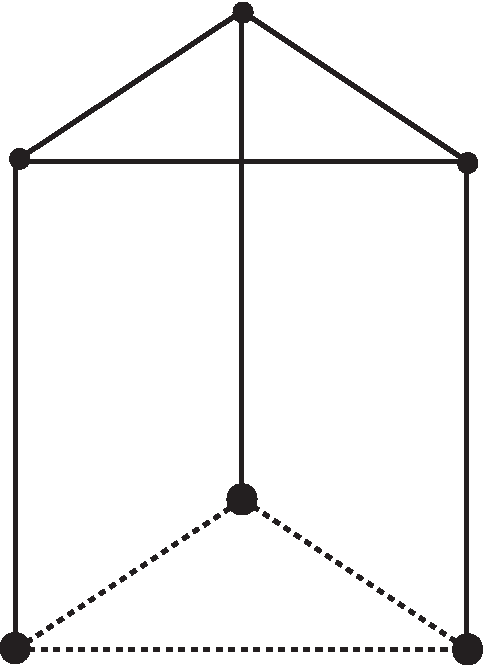
\includegraphics[width=0.7\textwidth]{images/35_15_6_56r2}\\
              \textit{[Fig. 2]}\\
              \clearpage
% Zeitz auskommentiert             %\vspace{0.5ex}
%              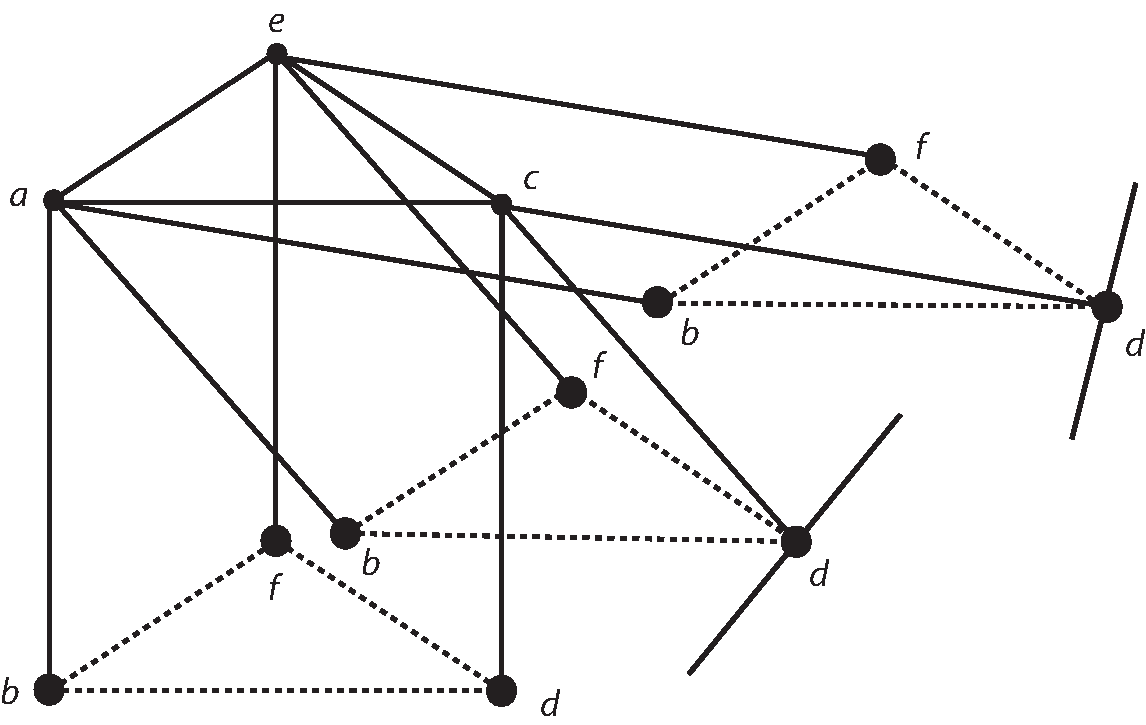
\includegraphics[width=0.6\textwidth]{images/35_15_6_56r4}\\
%              \textit{[Fig. 3]}
              \end{center}
              